%%%%%%%%%%%%%%%%%%%%%%%%%%%%%%%%%%%%%%%%%
% Thin Sectioned Essay
% LaTeX Template
% Version 1.0 (3/8/13)
%
% This template has been downloaded from:
% http://www.LaTeXTemplates.com
%
% Original Author:
% Nicolas Diaz (nsdiaz@uc.cl) with extensive modifications by:
% Vel (vel@latextemplates.com)
%
% License:
% CC BY-NC-SA 3.0 (http://creativecommons.org/licenses/by-nc-sa/3.0/)
%
%%%%%%%%%%%%%%%%%%%%%%%%%%%%%%%%%%%%%%%%%

%----------------------------------------------------------------------------------------
%	PACKAGES AND OTHER DOCUMENT CONFIGURATIONS
%----------------------------------------------------------------------------------------

\documentclass[a4paper, 11pt]{article} % Font size (can be 10pt, 11pt or 12pt) and paper size (remove a4paper for US letter paper)
\usepackage{color}
\usepackage[protrusion=true,expansion=true]{microtype} % Better typography
\usepackage{graphicx} % Required for including pictures
\usepackage{wrapfig} % Allows in-line images
\usepackage{endnotes}
\usepackage{mathpazo} % Use the Palatino font
\usepackage[T1]{fontenc} % Required for accented characters
\linespread{1.05} % Change line spacing here, Palatino benefits from a slight increase by default
\usepackage{fancyhdr}
\usepackage[margin=1.25in]{geometry}
\pagestyle{fancy}
\fancyhf{}
\rhead{Machine Learning Problem Set 1, 31.01.2019}
\lhead{Felix Adam}
\rfoot{Page \thepage}
\usepackage{amsmath}
\usepackage{amssymb}
\usepackage{version}
\usepackage{setspace}
\usepackage{enumerate}
\usepackage{multicol}
\usepackage{amsfonts}
\usepackage{amssymb}
\usepackage{graphicx}
\usepackage{rotating}
\usepackage{lscape}
\usepackage{pdflscape}
\usepackage{array,tabularx,float,dcolumn,lscape}
\usepackage{booktabs}
\usepackage{xr}
\usepackage{dcolumn}
\usepackage{hyperref} 
\usepackage{amsmath}
\usepackage{algorithm}
\usepackage[noend]{algpseudocode}
\graphicspath{ {../01_Figures/} }

\makeatletter
\def\BState{\State\hskip-\ALG@thistlm}
\makeatother

\newlength\tindent
\setlength{\tindent}{\parindent}
\setlength{\parindent}{0pt}
\renewcommand{\indent}{\hspace*{\tindent}}
\renewcommand{\familydefault}{\sfdefault}

\makeatletter
\renewcommand\@biblabel[1]{\textbf{#1.}} % Change the square brackets for each bibliography item from '[1]' to '1.'
\renewcommand{\@listI}{\itemsep=0pt} % Reduce the space between items in the itemize and enumerate environments and the bibliography

\renewcommand{\maketitle}{ % Customize the title - do not edit title and author name here, see the TITLE block below
\begin{flushright} % Right align
{\LARGE\@title} % Increase the font size of the title

\vspace{50pt} % Some vertical space between the title and author name

{\large\@author} % Author name
\\\@date % Date

\vspace{40pt} % Some vertical space between the author block and abstract
\end{flushright}
}

\begin{document}

\section{Mean Estimators} 

Compare the three mean estimators: empirical mean, trimmed mean and the median of means-estimator for thin- and heavy-tailed distribution. The performance should be measured as the probability of absolute deviation of the estimate $m_n$ from the true value $m$, $P\left( |m_n - m | > \epsilon \right)$

\subsection{Simulation Results}

\subsubsection{Standard Normal Distribution}

First, I simulate the performance of the three estimators on standard normally distributed data, for a range of $\epsilon$ and sample sizes.

\begin{figure}[H]
\centering
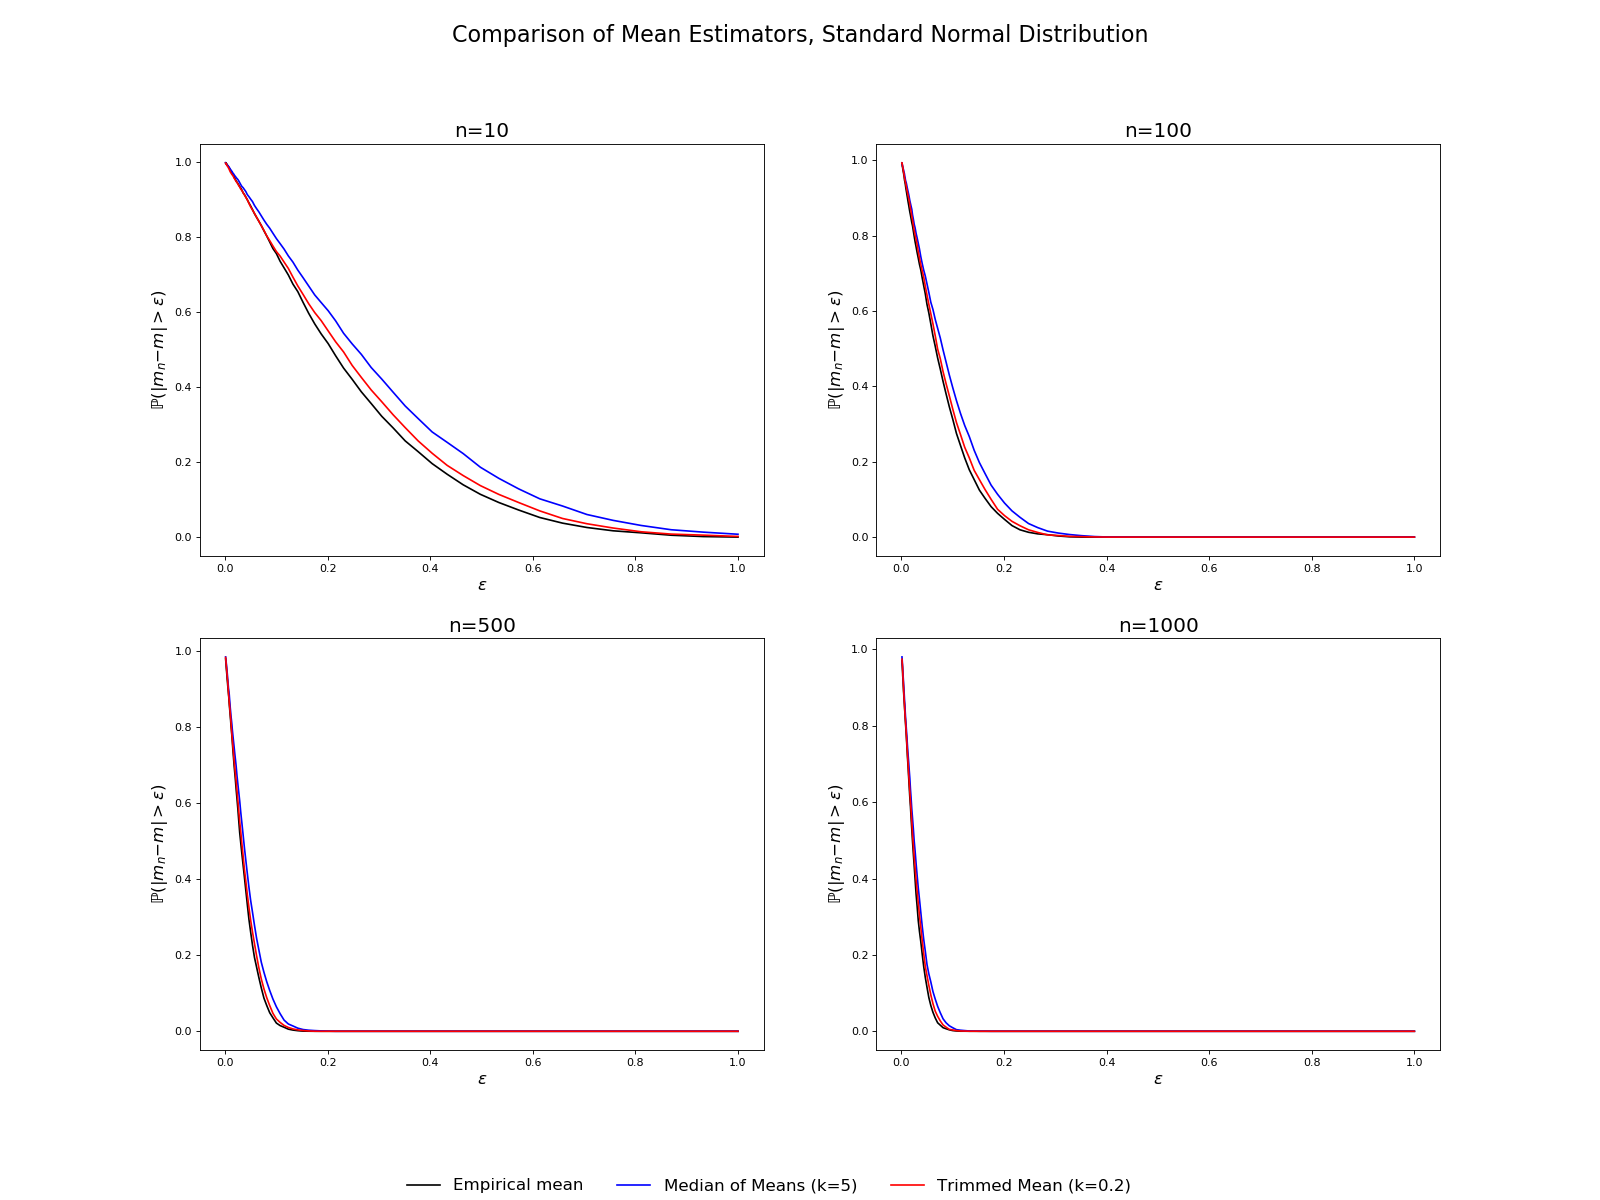
\includegraphics[scale= 0.3]{Gaussian_Base}
\end{figure}

\noindent The simulations show, that for all sample sizes, the empirical mean has the lowest probability of error for all $\epsilon$, followed by the trimmed mean and then the median of means. Further, as the sample size increases, the probability of high errors decreases for all estimators. \\

A look at the empirical distribution of $m_n - m$ reveals, that the empirical mean has the lowest variance among the three estimators, on standard normal data, followed by the trimmed mean and the median of means. Again, as the sample size increases, the variance of all estimators decreases. 

\begin{figure}[H]
\centering
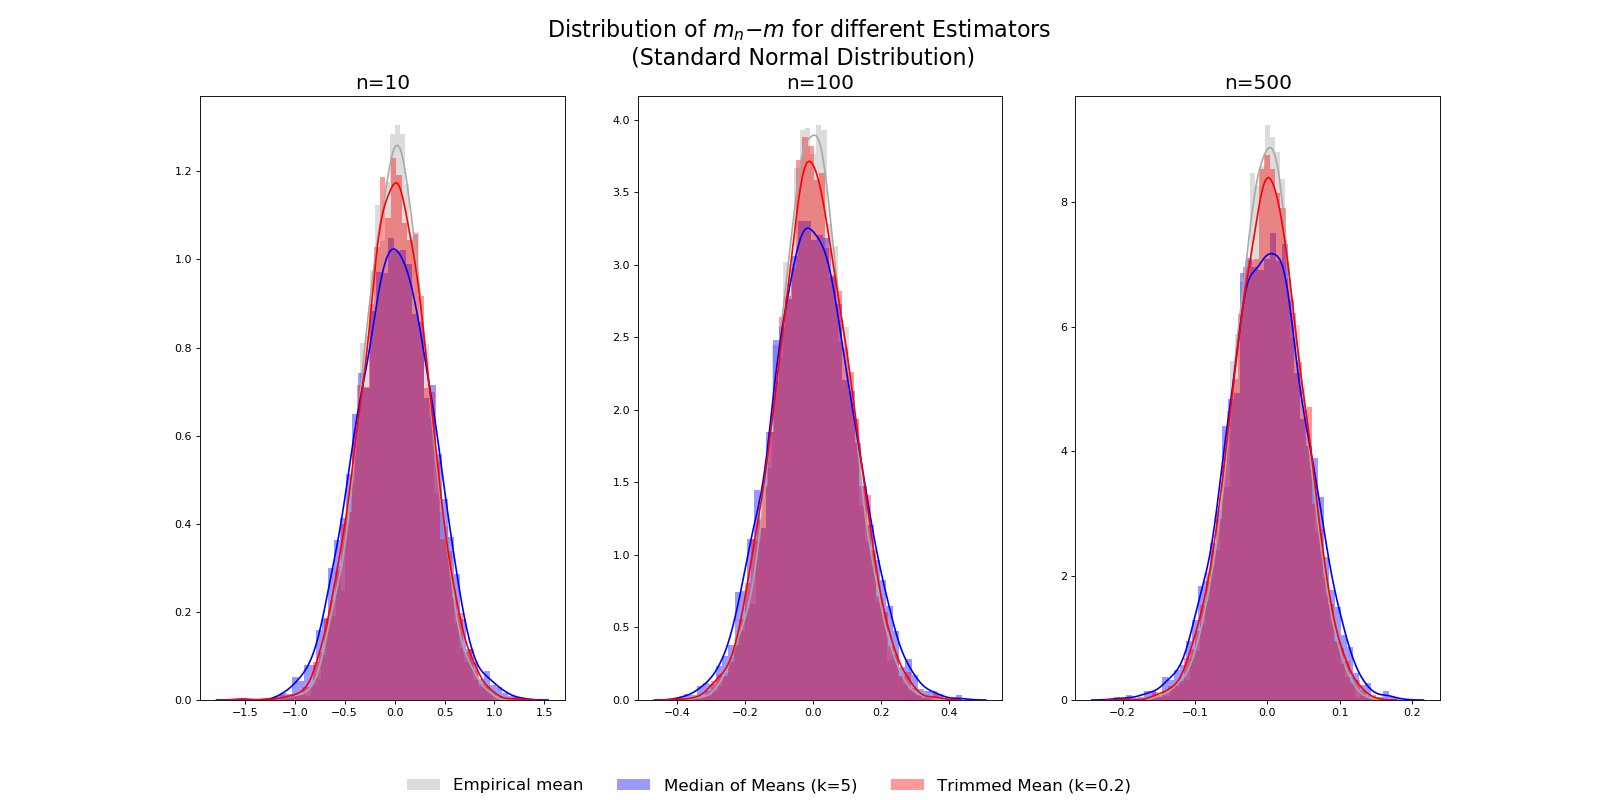
\includegraphics[scale=0.3]{Gaussian_Distribution_k5} 
\end{figure}

\noindent Varying the number of blocks for the median of means estimator and the percentage to be trimmed for the trimmed mean, we find for both estimators that the probability of error moves towards the probability of error of the empirical mean as the number of blocks and the percentage trimmed decreases. This is not particularly surprising, since the estimators are becoming more similar to the empirical mean with less blocks or smaller percentage trimmed.

\begin{figure}[H]
\centering
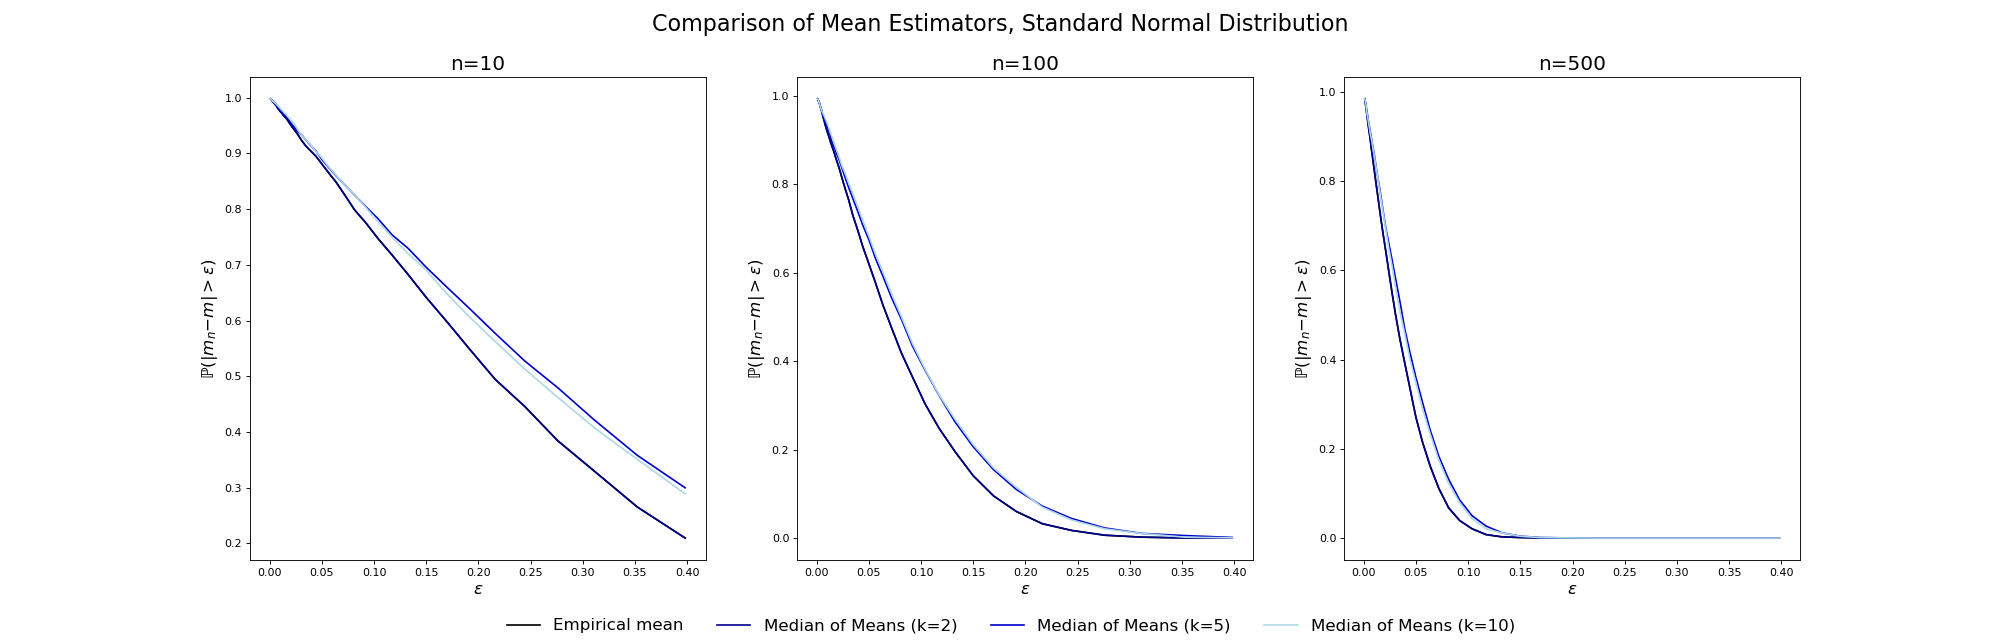
\includegraphics[scale=0.25]{Gaussian_MoM}
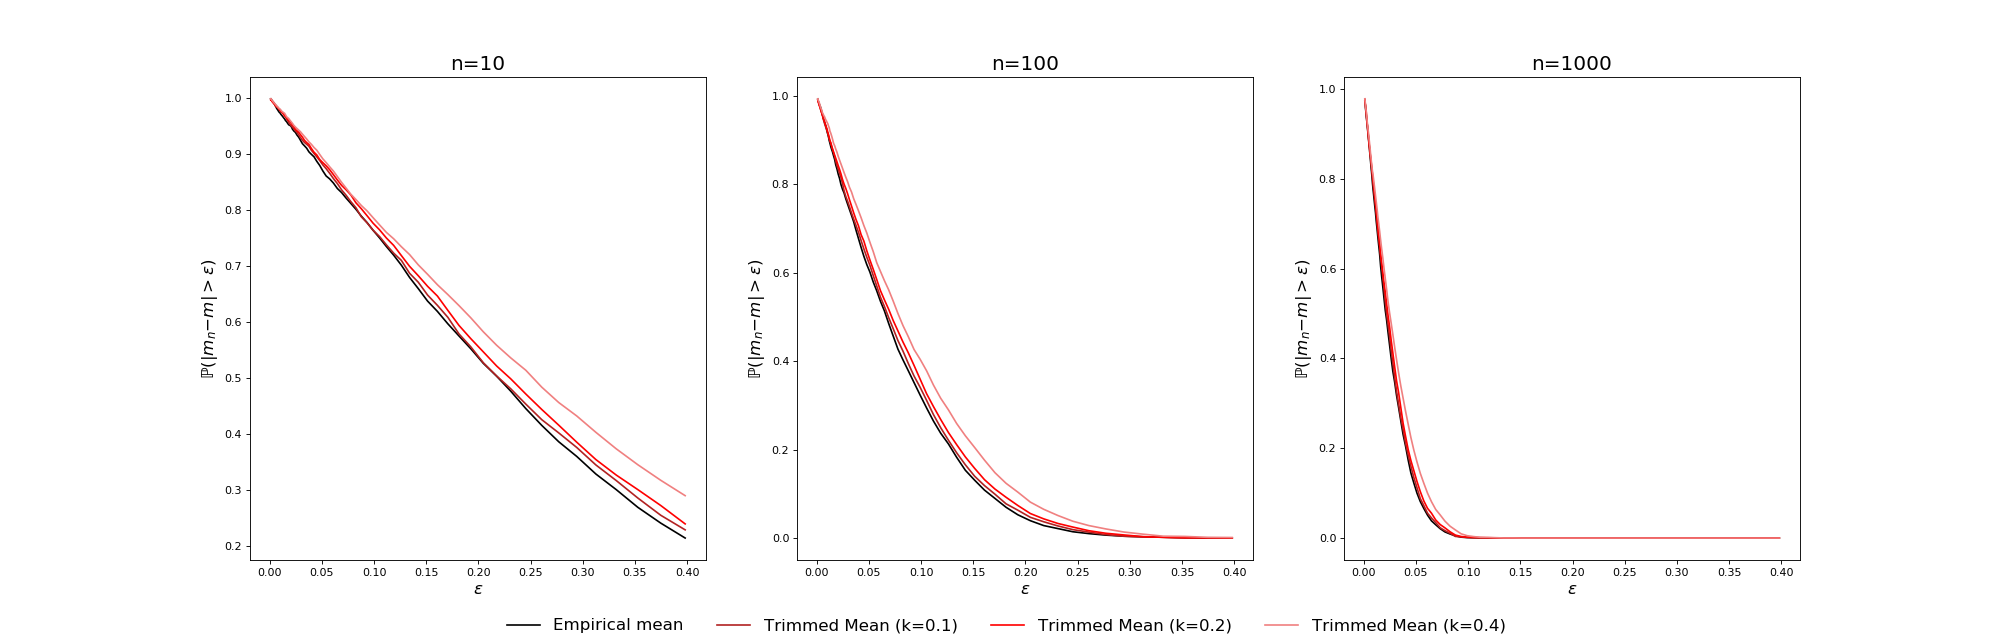
\includegraphics[scale=0.25]{Gaussian_TrM}
\end{figure}

\subsubsection{Student's t Distribution}

Having shown, that the empirical mean works best for a thin-tailed distribution like the standard normal, I will now simulate the performance of the estimators on the t-distribution with varying degrees of freedom.

\begin{figure}[H]
\centering
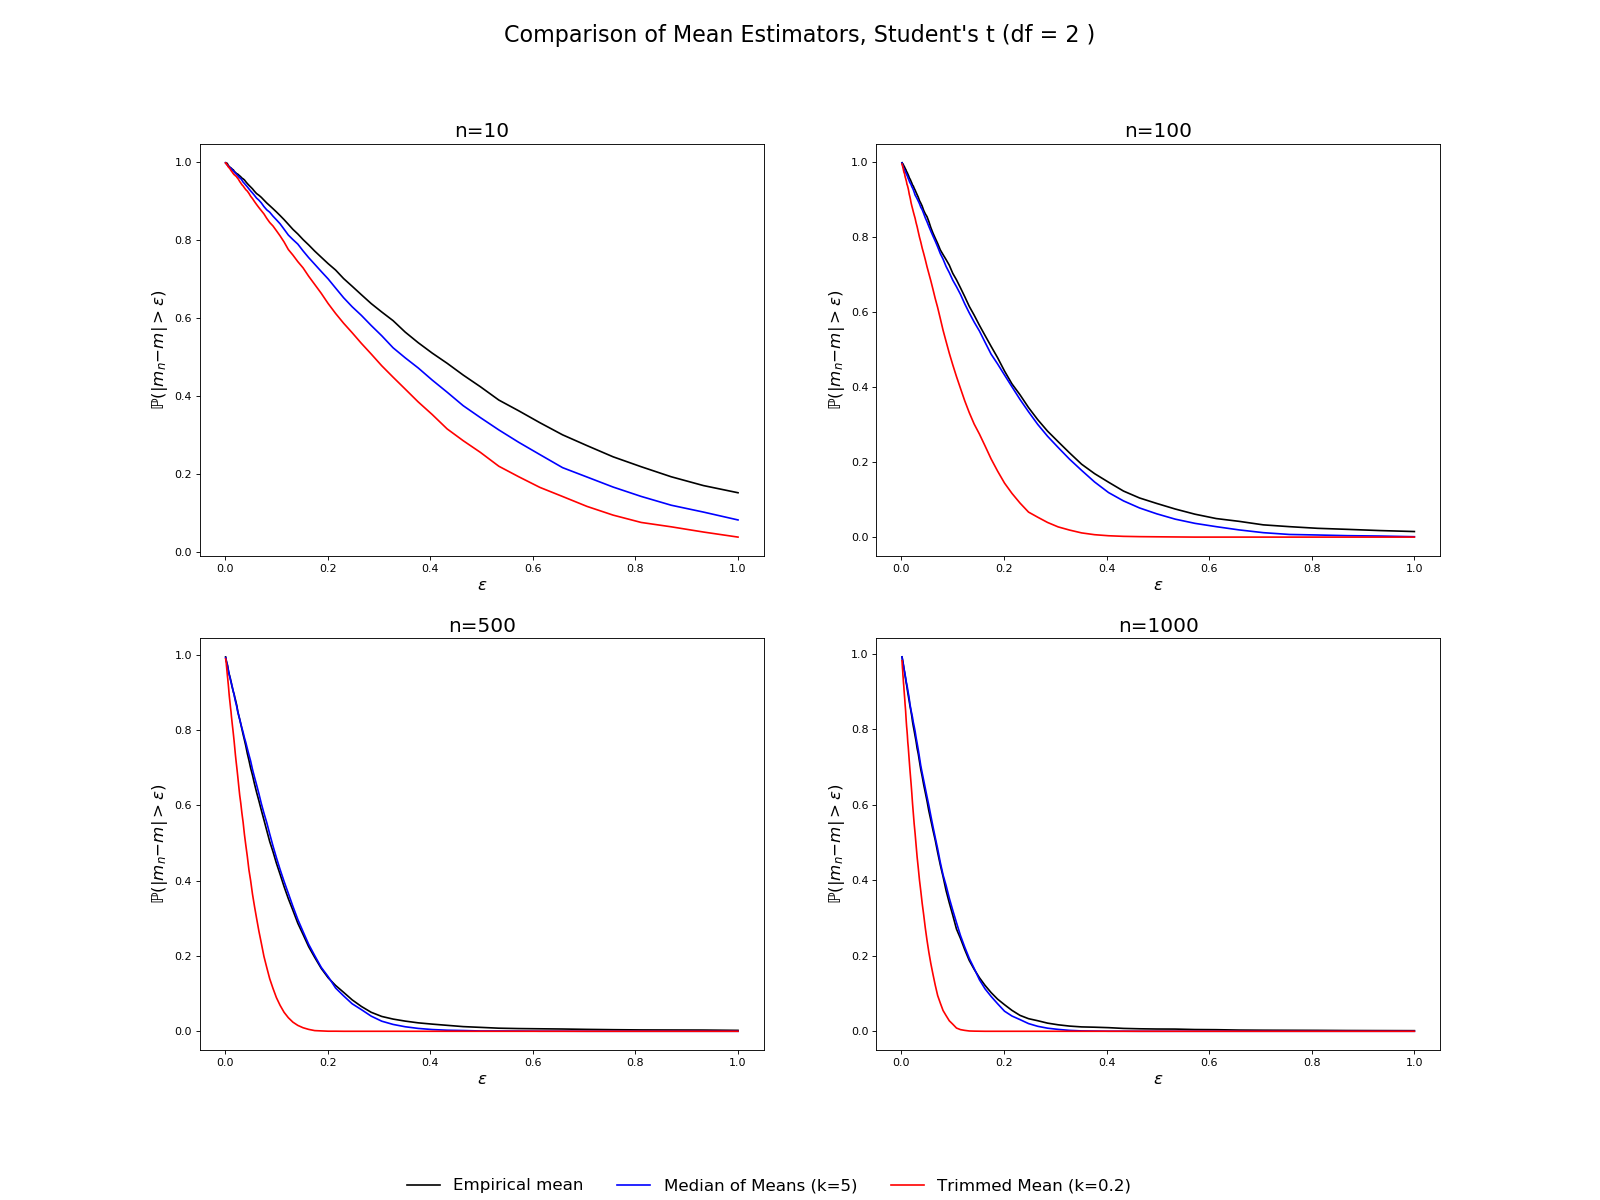
\includegraphics[scale=0.3]{Students_2df}
\end{figure}

\noindent The results show, that the mean estimator has now the highest probability of error, followed by the median of means and then the trimmed mean. This is particularly pronounced for smaller sample sizes. As before, as the sample size increases, the probability of error decreases. What about the distribution of the errors?

\begin{figure}[H]
\centering
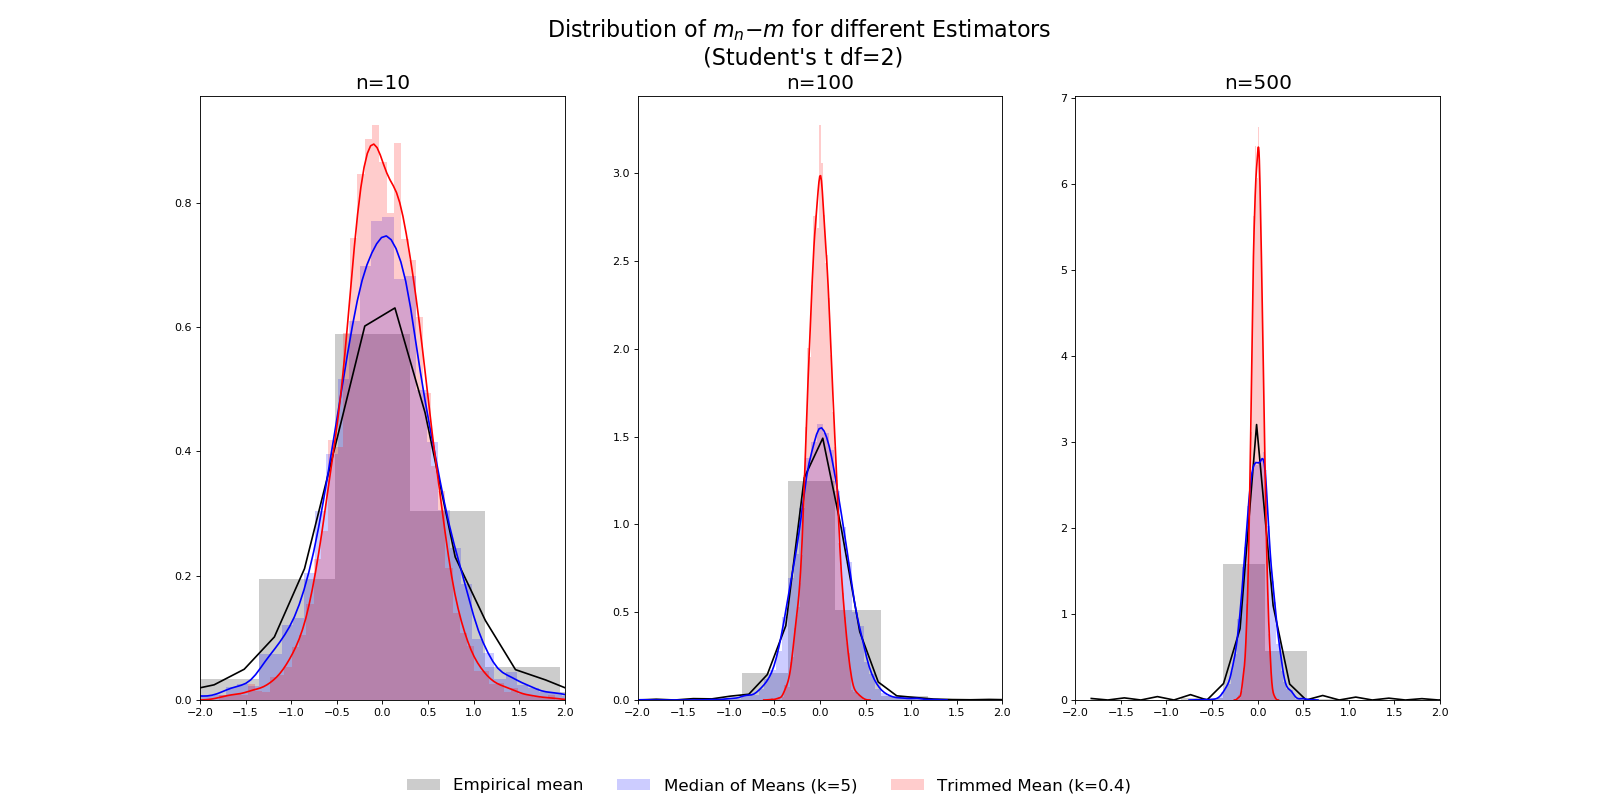
\includegraphics[scale=0.25]{Studentsdf2_Dist_k5}
\end{figure}

In smaller samples, the distribution of the error of the empirical mean has heavier tails than the trimmed mean and median of means. This is even true for larger sample sizes, but not as pronounced. The median of means has a slightly higher variance of $m_n -m$ compared to the trimmed mean. \\

Further, as the degree of freedoms increase, the probability of error for all estimators decreases, however it decreases more for the empirical mean than for the others, since the t-distribution converges to a normal distribution as the degrees of freedom increase.

\begin{figure}[H]
\centering
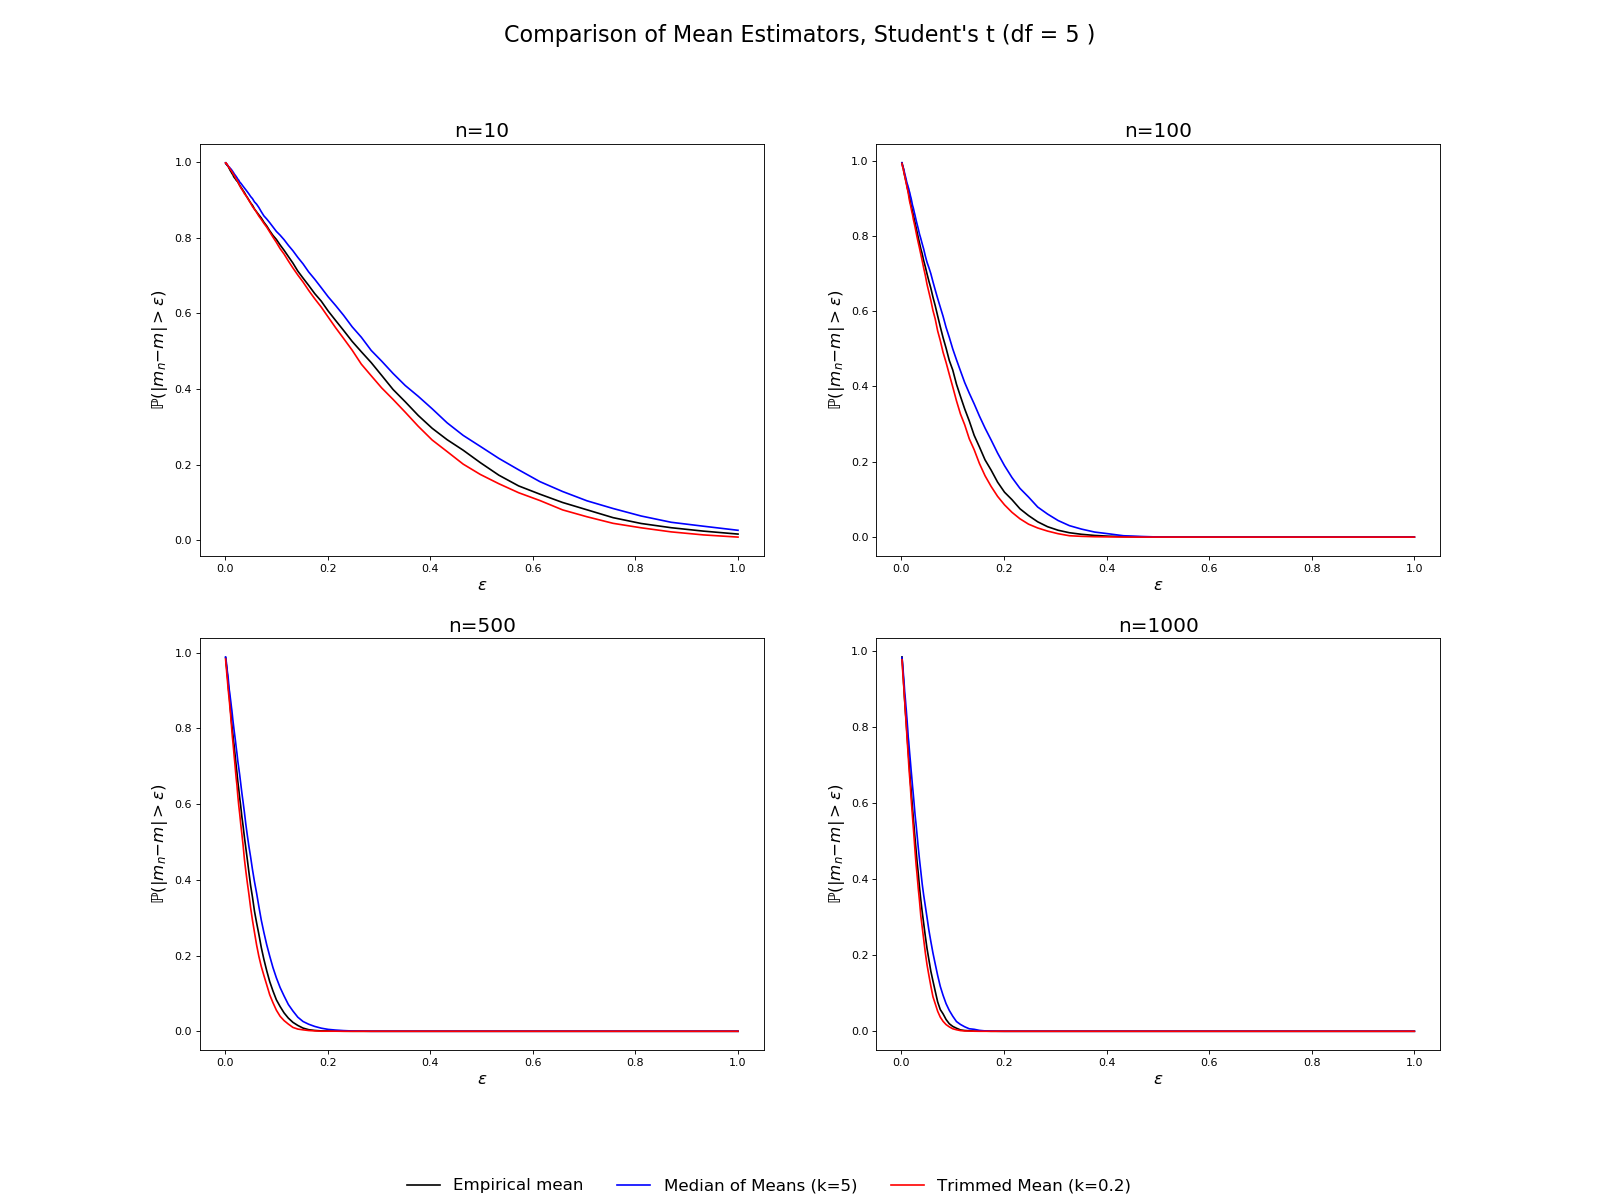
\includegraphics[scale=0.29]{Students_5df}
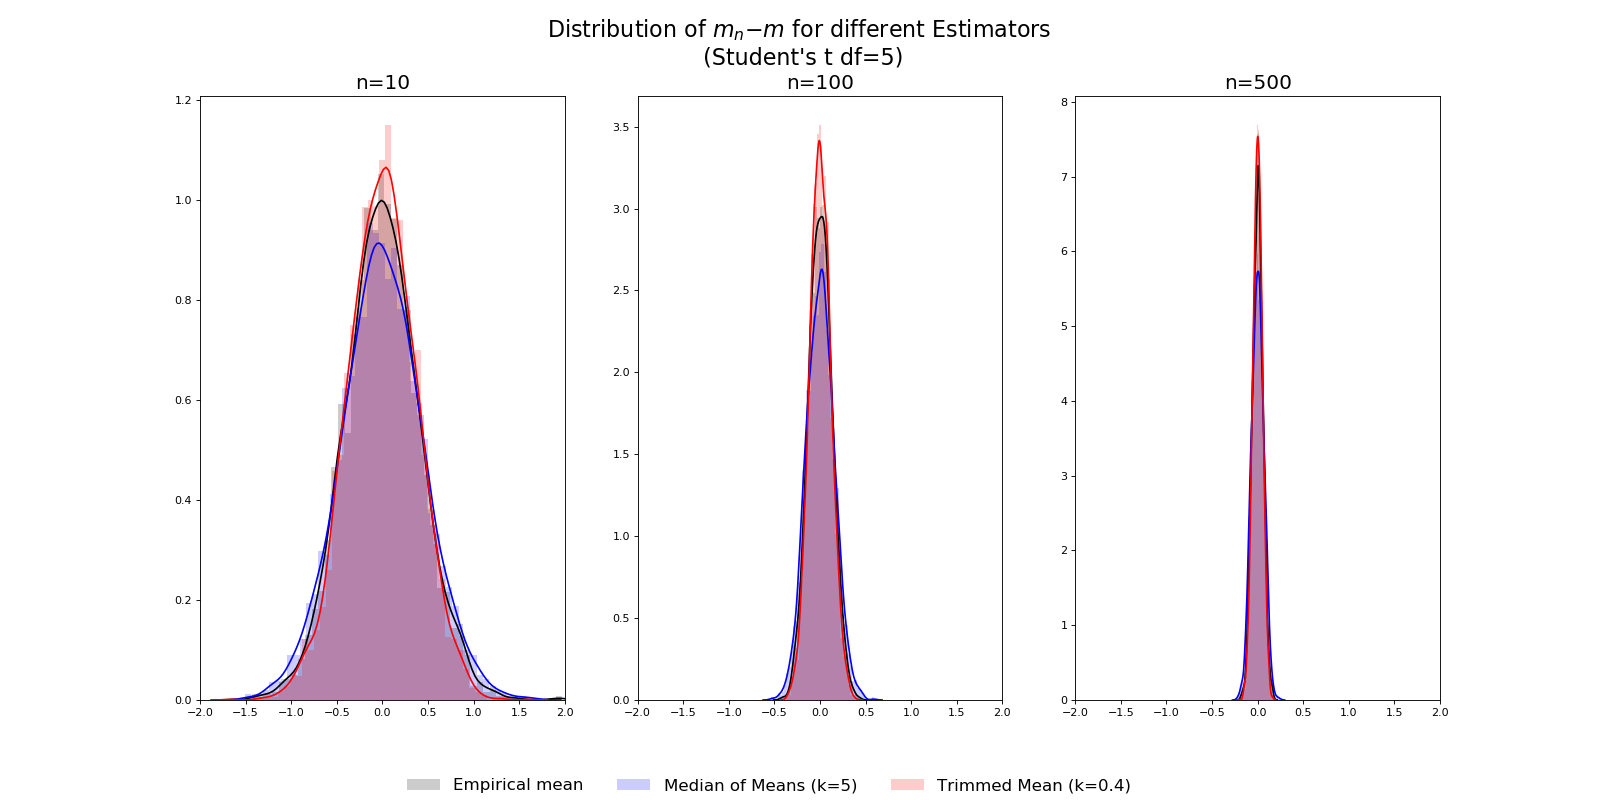
\includegraphics[scale=0.29]{Studentsdf5_Dist_k5}
\end{figure}

What about varying block size and trimm?

\begin{figure}[H]
\centering
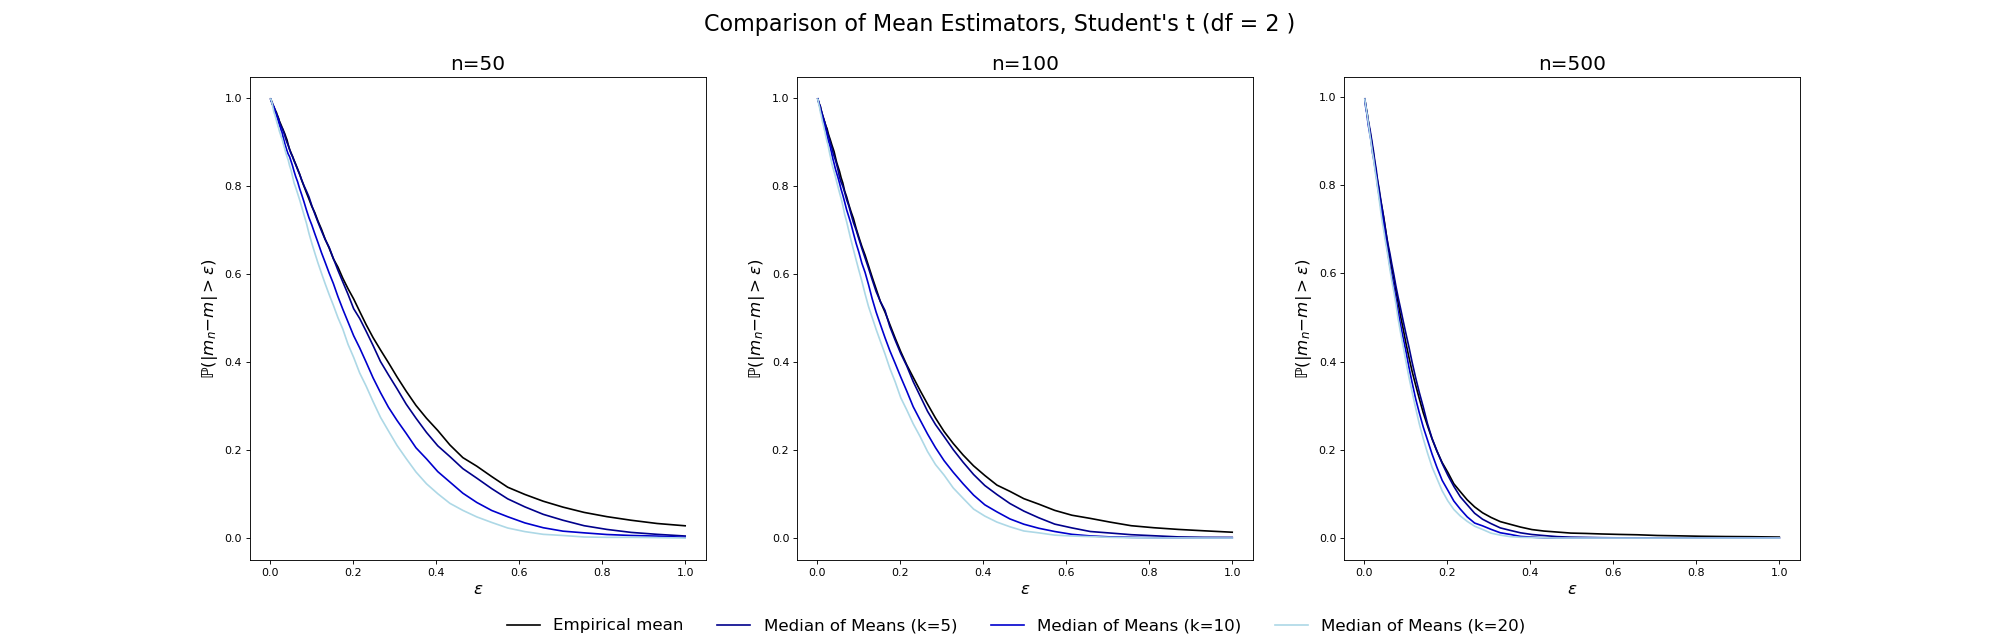
\includegraphics[scale=0.25]{Students_MoM_2df}
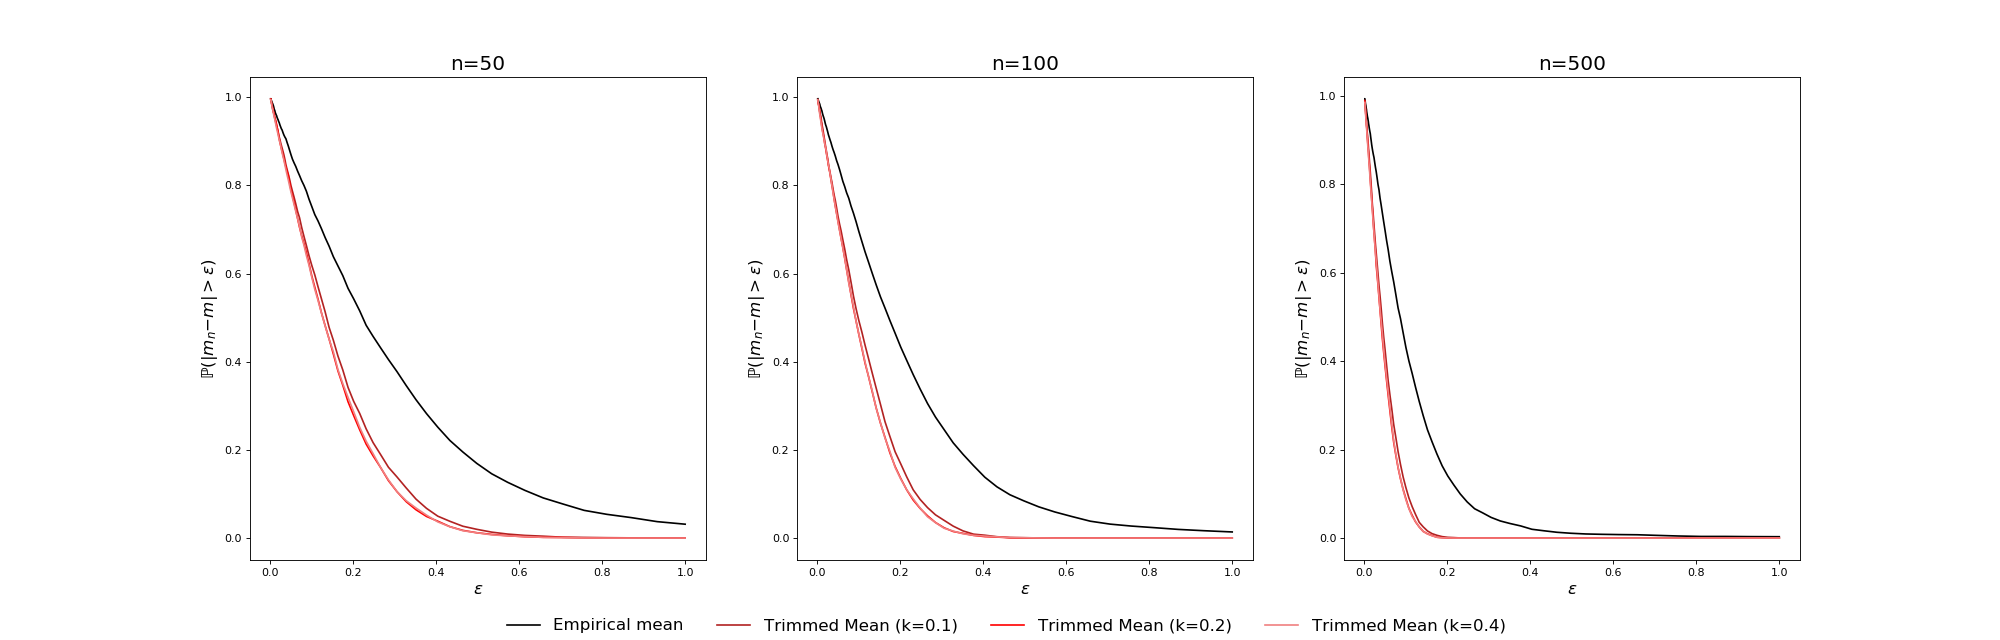
\includegraphics[scale=0.25]{Students_TrM_2df}
\end{figure}

As the number of blocks increases, the performance of the median of mean estimator increases, indicated by lower error probabilities. Similarly, the performance of the trimmed mean increases with a higher percentage of data trimmed. For both estimators, the differences across block size and number of points trimmed decreases with larger samples. 


\section{Cosine of Random Vectors}

Let $X$ be a random vector uniformly distributed in the d-dimensional cube $[-1, 1]^d$ (i.e., the components of $X = (X_1 . . . , X_d)$ are independent, uniformly distributed in the interval $[-1, 1])$. What can you say about the distribution of $||X||^2$? Determine the mean, the variance, and establish concentration inequalities.\\
\\
If $X'$ is another independent vector drawn from the same distribution, what is the typical
order of magnitude (as a function of $d$) of the cosine of the angle between $X$ and $X'$? Recall that the cosine of the angle between two vectors $u$ and $v$ is

$$\frac { u ^ { T } v } { \| u \| \cdot \| v \| }$$


\subsection{Distribution and Concentration Inequalities}

First, we note that the entries of the vector $X$ are i.i.d. $Unif[-1,1]$ and have expectation $E[X_i] = 0$ and variance $\text{Var}(X_i)= \frac{1}{3}$. We can use these properties to derive the mean and variance of $||X||^2$. Note that throughout this section, $d$ denotes the number of dimensions of the vector $X = (X_1, ... , X_d)$

\subsubsection{Expected Value}

We note that $||X||^2 = \sum_{i=1}^n X_i^2$ for all $i$. Further, $E[X_i^2] = \text{Var}[X_i] - (E[X_i])^2 = \frac{1}{3}$. Therefore, by independence and the identical distribution, the expected value is

\begin{equation*}
E[||X||^2] = E[\sum_{i=1}^d X_i^2] = \sum_{i=1}^d E[X_i^2] = d E[X_1^2] = \frac{d}{3}
\end{equation*}

The expected value of the squared norm grows with the number of dimensions $d$.

\subsubsection{Variance}

The variance can be derived using a similar argument. 

\begin{equation*}
\text{Var}(||X||^2) = \text{Var} \left(\sum_{i=1}^d X_i^2 \right) = \sum_{i=1}^d \text{Var}(X_i^2) 
\end{equation*}

I can derive $\text{Var}(X_i)$ using $E[X_i^4] = 1/5  \sum_{i=0}^4 (-1)^i (1)^{4-i}$.
 
\begin{equation*}
\begin{split}
Var[X_i^2] &= E[(X_i^2)^2] - \left( E[X_i^2] \right)^2 \\
&= E[X_i^4] - \frac{1}{9} \\
&= \frac{1}{5} - \frac{1}{9} = \frac{4}{45} 
\end{split}
\end{equation*}

Plugging this into the pervious equation we get

\begin{equation*}
\text{Var}(||X||^2) = \sum_{i=1}^d \frac{4}{45} = d\frac{4}{45}
\end{equation*}

Therefore, the variance of $||X||^2$ also grows with the number of dimensions. 

\subsubsection{Concentration Inequalities}

Having derived the mean and variance, we can now establish some concentration inequalities.\\

\textbf{Markov's Inequality}

\begin{equation*}
P(||X||^2 \geq t) \leq \frac{E \left[||X||^2 \right]}{t} = \frac{d}{3t}
\end{equation*}


\textbf{Chebyshev's Inequality}

\begin{equation*}
P(||X||^2 - E\left(||X||^2 \right) \geq t) \leq \frac{\text{Var}(||X||^2)}{t^2} = \frac{4d}{45t^2}
\end{equation*}

\newpage

\textbf{Chernoff Bounds}

Since $X_i^2 \in [0,1]$, I can use Hoeffdings Lemma to derive the Chernoff bound for $\|X \|^2$


\begin{align*}
P(||X||^2 - E\left(||X||^2 \right) \geq t) = P \left( \sum_{i=1}^n X_{i}^2 - \frac{1}{3} \right)  &\leq \frac{E\left(e^{ \lambda( \sum_{i=1}^n X_{i}^2 -  \frac{1}{3} )} \right)}{e^{\lambda t} } \\
 	&\leq \frac{E \left( e^{ \lambda (X_1^2 -1/3} \right)^n}{e^{\lambda t }} \\
 	&\leq \frac{e ^{n\lambda^2 / 8}}{e^\lambda t} 
\end{align*}

Optimizing the last expression with respect to $\lambda$ we get $\lambda^* = \frac{4t}{n}$. This leads to the following bound

\begin{equation*}
P(||X||^2 - E\left(||X||^2 \right) \geq t) \leq e^{-2t^2 / 2} 
\end{equation*}

\subsection{Cosine}

Having established some propertis of $||X||^2||$ we can make statments about the order of magintude of the cosine of the angle $\alpha$ between the two random vectors $X$ and $X'$ which have both values from a Uniform distribution with parameters $[-1,1]$. 

\subsubsection{Order of Magnitude of the  Cosine}

\begin{equation*}
E \left[ \cos(\alpha) \right] = E \left[ \frac{X^TX'}{ \| X \| \cdot \| X' \|} \right]
\end{equation*}

Even though we can't assume independence between the numerator and denominator, we will first check the expected value of the denominator and see whether it will deviate much from it's expected value. By the i.i.d. property of $X$ and $X'$ we can write

\begin{equation*}
E[\| X \| \cdot \| X' \|] = E[ \|X \|^2] = \frac{d}{3}
\end{equation*}

Plugging this into the cosine we get 

\begin{equation*}
E \left[ \frac{X^TX'}{ \| X \| \cdot \| X' \|} \right] = \frac{3}{d} E \left[ \sum_{i=1}^d X_i X_i' \right] = \frac{3}{d}  \sum_{i=1}^d E[X_i] E[X_i'] = 0
\end{equation*}

by using independence and $E[X_i] = E[X_i'] = 0$. 

Therefore, the expected value of the cosine between the two vectors is 0. 
The question is now, how sure can we be, that the cosine will be close to zero, given the number of dimensions $d$. We can derive the variance of the cosine in order to get an estimate of the order

\subsubsection{Variance of the Cosine}

\begin{align*}
\text{Var}(\cos(\alpha)) &= \text{Var} \left( \frac{3}{d}  \sum_{i=1}^d X_i X_i' \right) \\
&= \frac{9}{d^2}  \sum_{i=1}^d \text{Var}(X_i X_i') \\
&=  \frac{9}{d}  \text{Var}(X_1) \text{Var}(X_2) = \frac{9}{d} (\text{Var}(X_1))^2  \\
&= \frac{9}{d} \cdot \frac{1}{9} = \frac{1}{d}
\end{align*}

by independence and identity of the entries of $X$ and $X'$. Therefore, the higher the dimension, the more certain we can be that the cosine between the two random vectors will be close to zero. Using the standard deviation, the order of magintude of the cosine is therefore $O(\frac{1}{\sqrt(d})$. The higher the dimension of the two random vectors, the more likely it will be, that the cosine is close to zero. 

\newpage

\section{Chernoff Bounds}
Let $X_1, . . . , X_n$ be i.i.d. non-negative random variables with mean $E[X_1] = m$ and
second moment $E[X_1^2] = a^2$. Use the Chernoff bound to prove that, for all $t \in (0, m)$,

\begin{equation*}
\mathbf { P } \left\{ \frac { 1 } { n } \sum _ { i = 1 } ^ { n } X _ { i } < m - t \right\} \leq e ^ { - n t ^ { 2 } / \left( 2 a ^ { 2 } \right) }
\end{equation*}

\subsection{Proof}

First, we multiply each side with $-n$ and then apply the generic Chernoff bound. Further we use the hint and $1+x \leq e^x$.

\begin{align*}
P \left( \frac { 1 } { n } \sum _ { i = 1 } ^ { n } X _ { i } < m - t \right) &= P \left( - \sum _ { i = 1 } ^ { n } X _ { i } \geq n ( t - m ) \right) \\
&\leq \frac{E \left( e ^{-\lambda \left(\sum_{i=1}^n X_i \right) } \right)}{e^{\lambda n(t-m)}} \\
&\leq \frac{E \left( e ^{-\lambda \left(\sum_{i=1}^n X_i \right) } \right)}{e^{\lambda n(t-m)}} \\
&\leq \frac{E \left( e ^{-\lambda X_1^2 } \right)^n}{e^{\lambda n(t-m)}} 
\leq  \frac{E \left( 1 - \lambda X_1 + \frac{\lambda^2 X_i^2}{2}   \right)^n}{e^{\lambda n(t-m)}} \\
&\leq \frac{ \left(1 - \lambda m + \frac{\lambda^2 a^2}{2} \right)^n  }{e^{\lambda n(t-m}} \\
&\leq \frac{e^{- n\lambda m + \frac{n\lambda^2 a^2}{2} }}{e^{\lambda n(t-m)}} \\
&\leq e^{\frac{n \lambda^2 a^2}{2}- \lambda n t }
\end{align*}

Now we can optimize the exponent with respect to $\lambda$. After taking the derivative we get
\begin{equation*}
\lambda a^2 -t = 0 <=> \lambda^* = \frac{t}{a^2}
\end{equation*}

We then plug this into the previous equation and get 

$$P \left( \frac { 1 } { n } \sum _ { i = 1 } ^ { n } X _ { i } < m - t \right) \leq e^{ \frac{-n t^2 }{a^2} + \frac{t^2}{a^4} a^2 n/2 } = e ^ { - n t ^ { 2 } / \left( 2 a ^ { 2 } \right) }$$

\newpage

\section{Random Projections}

Write a program that projects the $n$ standard basis vectors in $\mathbb { R } ^ { n }$ to a random 2-dimensional subspace. Compare the outcome to standard normal points.

\subsection{Simulation Results}
\begin{figure}[H]
\centering
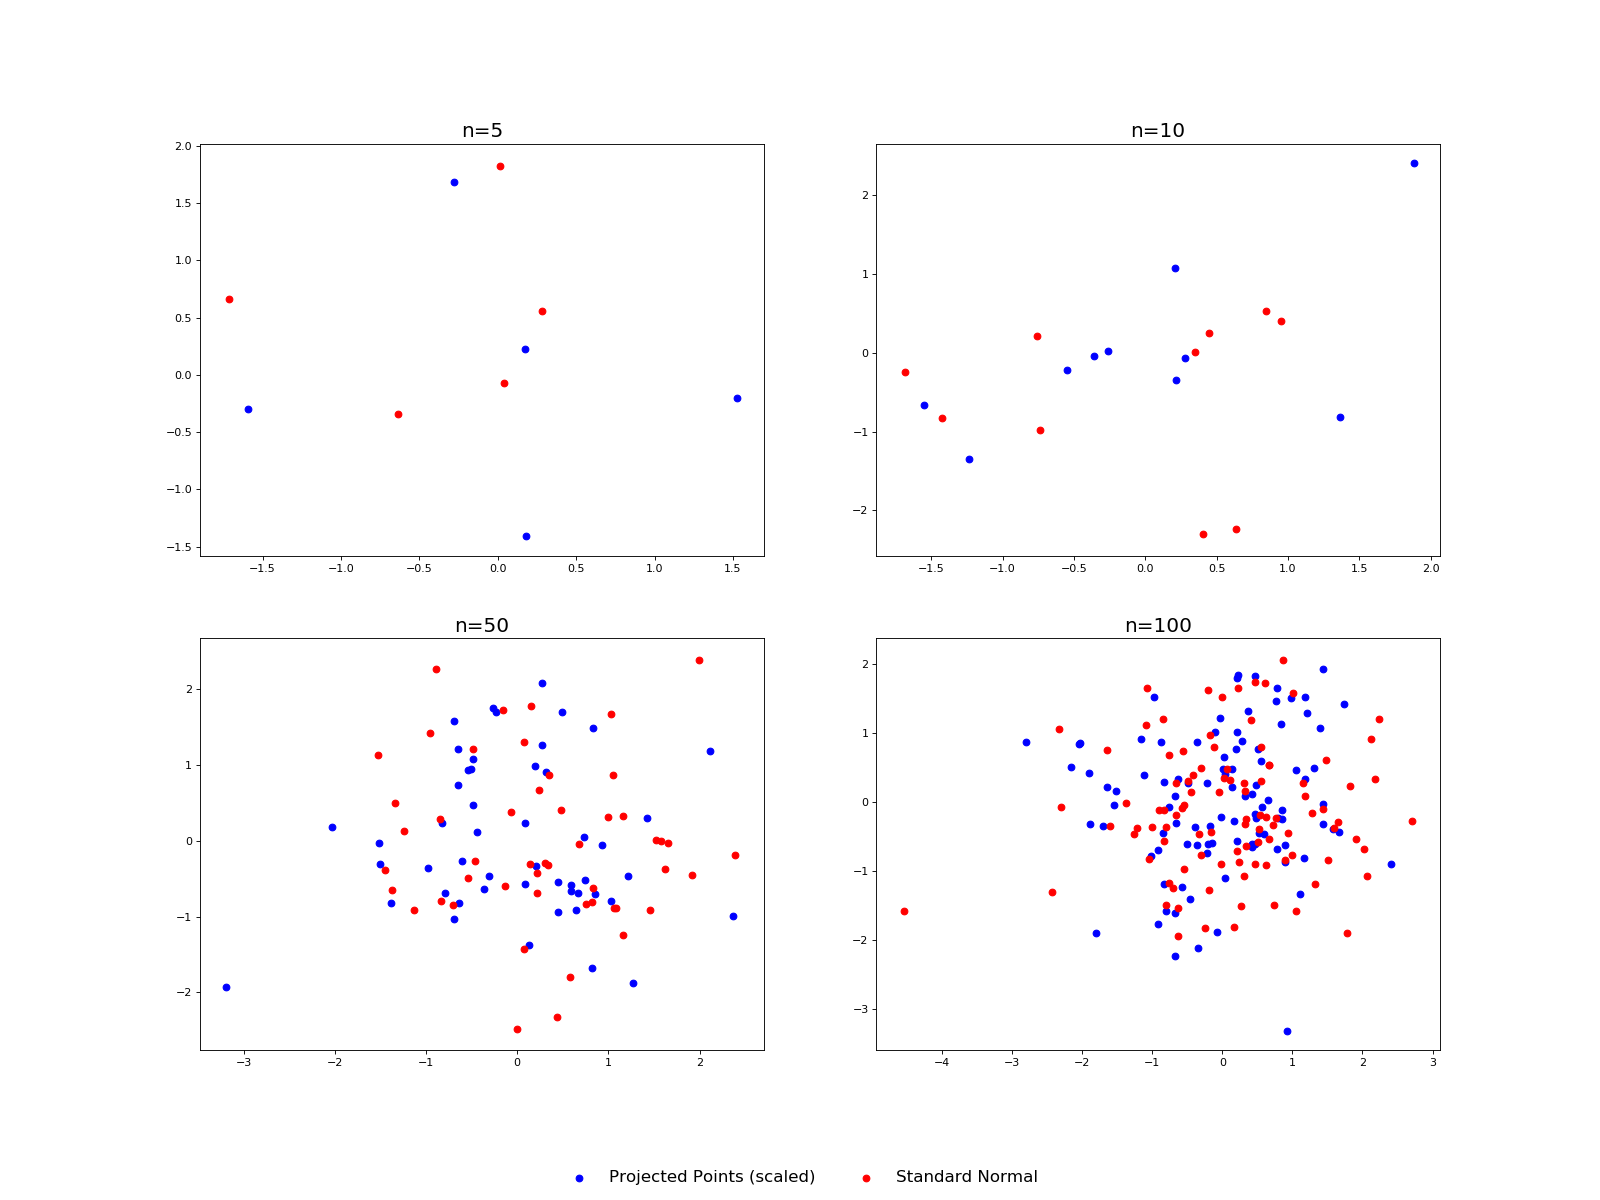
\includegraphics[scale=0.25]{Random_Projections1}
\end{figure}
\begin{figure}[H]
\centering
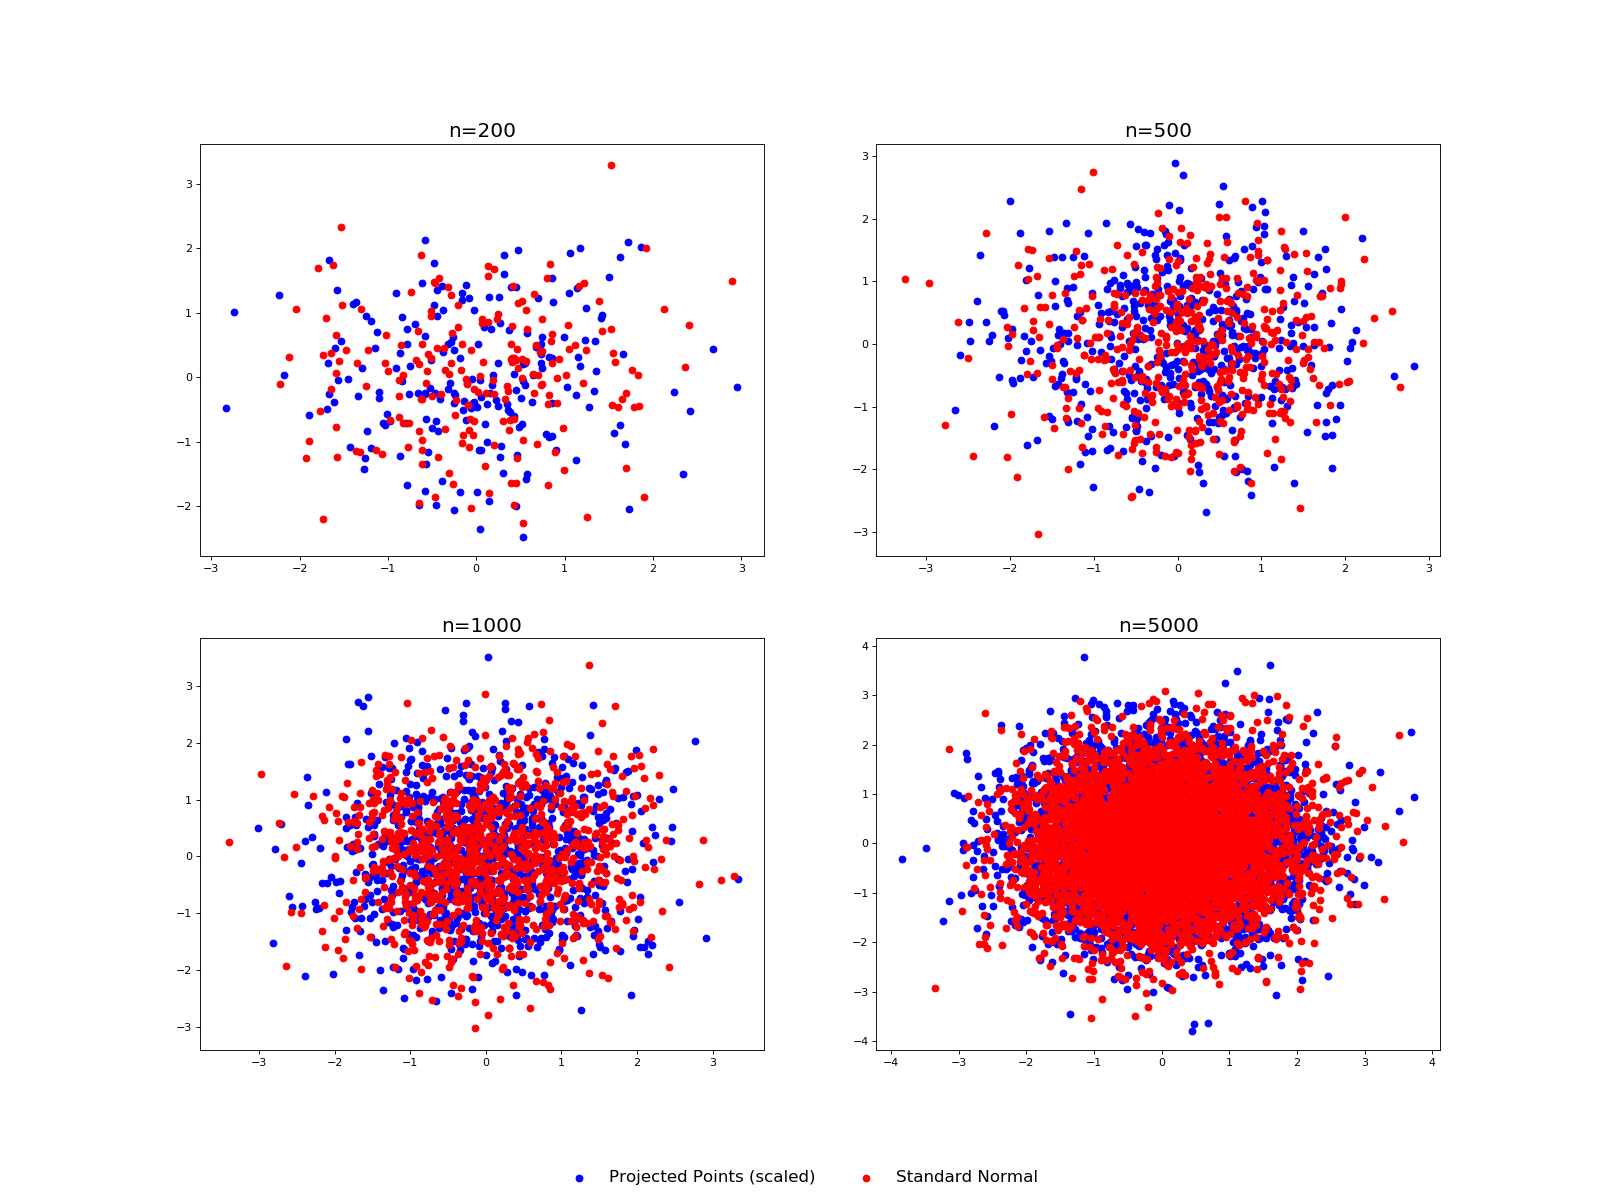
\includegraphics[scale=0.25]{Random_Projections2}
\end{figure}

The projected points resemble a multivariate standard normal distribution, as n grows. This is not entirely surprising, as we're basically multiplying the n x n identity matrix with a random matrix of size n x 2. Further, with larger n, we see less and less structure in the projected points. Basically, there are no apparent differences between the projected (blue) and the random (red) points as $n$ increases. \\

What about the distances between the projected points, relative to the distance before the projection? Before the projection, the distance between two basis vectors is always $\sqrt{2}$. The Johnson-Lindenstrauss Lemma tells us, that we can map a set of $n$ points from a space $\mathbb{R}^D$ to a subspace $\mathbb{R}^d$ ($f: \mathbb{R}^D \rightarrow \mathbb{R}^d$) , such that 

\begin{equation*}
1- \epsilon \leq \frac{\| f(a) - f(b) \|^2}{\| a - b \|^2} \leq 1 + \epsilon
\end{equation*}

as long as 

$$d \geq \frac{8\log(n)}{\epsilon^2}$$

In this case we'll always have $n$ points since we're projecting the basis vectors of $\mathbb{R}^n$ on $\mathbb{R}^2$. So we can say that our error $\epsilon$ grows with the number of dimensions, since we're not getting more data-points, just more dimensions.

$$\epsilon \geq \sqrt{4 \log(n)}$$

Consequently, with increasing $n$ it becomes harder and harder to project the points into $\mathbb{R}^2$, if we want to keep the error low.

\end{document}


 